
\section{اطلاعات توسعه}

مستند فنی شامل اصلاعاتی از فرآیند توسعه نیز می‌باشد. این اطلاعات شامل تاریخ
تغییرات، توسعه دهنده‌گان نسخه و یا مواردی است که کاربران را در به کارگیری و یا
دنبال کردن تغییرات یاری می‌کند.
گرچه این اطلاعات در نگاه نخست بسیار کم و بی اهمیت است اما وابستگی میان زیر
سیستم‌ها را تعیین می‌کند.
برای نمونه تصور کنید که یک فراخوانی جدید در بسته از نسخه 1.0.1 ایجاد شده است، در
این صورت برای به کارگیری زیرد سیستم‌ها و یا بسته‌هایی که از این فراخوانی استفاده
می‌کنند باید نسخه معادل و یا بالاتر از آن در دسترس باشد.

\subsection{تاریخ}
% date

% Starts a paragraph where one or more dates may be entered.
تاریخ عبارت است از یک پاراگراف کامل که رویدادهای متفاوت و زمان آنها را تعیین
می‌کند.
به عنوان نمونه فرض کنید که در تاریخی معین پیاده سازی یک تابع به روز شده است تا
با ذخیره نتایج جستجوهای قبل، جستجوهای بعدی را سریع‌تر انجام دهد.
این موضوع را می‌توان با استفاده از برچسب تاریخ به مستند تابع اضافه کرد.
ساختار کلی این برچسب به صورت زیر است.

\begin{C++}
/**
 * \date {date description}
 */
\end{C++}

این برچسب پاراگراف بعد از خود را به عنوان متنی در نظر می‌گیرد که رویدادهای
متفاوت را تشریح می‌کند.
این متن از ساختارهای داخلی خاصی حمایت نمی‌کند و تمام امکانات در نظر گرفته شده
برای نمایش مناسب متن نیز در آن قابل استفاده است.
متن این برچسب با رسیدن به یک خط خالی و یا بخش دیگر پایان می‌یابد.

گرچه می‌توان تمام رویدادها را با استفاده از یک برچسب و تنها در یک پاراگراف بیان
کرد، اما بهتر است که از چندین برچسب برای این کار استفاده کرد.
زمانی که برچسب‌ها به صورت متوالی در مستند ظاهر شده باشد در حروجی با هم ترکیب شده
و در یک قسمت اما در خط‌های متوالی نمایش داده می‌شوند.
برای نمونه فرض کنید که دو رویداد در سالهای 1387 و 1390 رخ داده است، در این صورت
این دو را می‌توان به صورت زیر مستند کرد:

\begin{C++}
/**
 * \brief date example
 *
 * \date Search algorithm is update in 1387.
 * \date History is added in 1390.
 */
int search(string str);
\end{C++}

خروجی تولید شده برای این مستند در شکل
\ref{write/document-the-code/developer-info/date-multi} نمایش داده شده است.
همانگونه که در این شکل قابل مشاهده است، تمام رویدادها به صورت متوالی و در خط‌های
جدا آورده شده و نمایش مناسبی را برای آنها ایجاد کرده است.
\begin{figure}
	\centering
	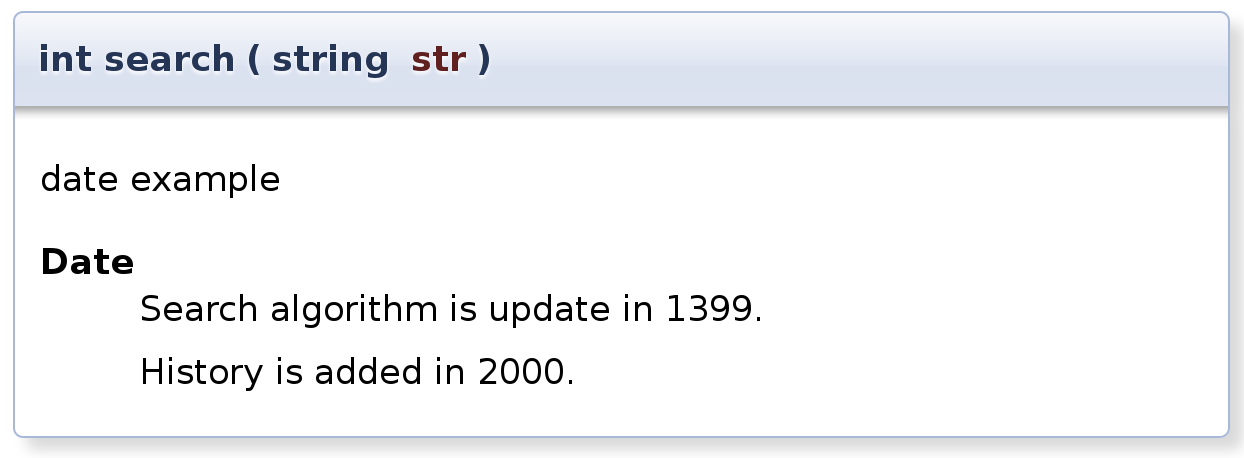
\includegraphics[width=0.8\textwidth]{image/write/document-the-code/developer-info/date-multi}
	\caption[چند برچسب تاریخ]{
		استفاده از چندین برچسب تاریخ پشت سر هم.
	}
	\label{write/document-the-code/developer-info/date-multi}
\end{figure}


\subsection{نسخه}
% version 
% \version { version number }

در پروژه‌های نرم‌افزاری، تغییراتی ایجاد شده در هر بسته با استفاده از یک شماره
مرز بندی می‌شود که به آن نسخه می‌گویند.
برای نمونه فرض کنید که در طول زمان چهار ویژگی به یک بسته نرم‌افزاری اضافه شده
است، یک مرزبندی این است که دو ویژگی در نسخه شماره ۱ و دو ویژگی دگر در نسخه شماره
۲ قرار گیرد.
در نسخه بندی یک سیستم، ترتیب صعودی میان نسخه‌ها به منزله پیشرفت پروژه در نظر
گرفته می‌شود.
در نمونه اورده شده نیز بعد از نسخه شماره ۲ تمام چهار ویژگی در سیستم وجود خواهد
داشت در حالی که نسخه شماره ۱ تنها شامل دو ویژگی است.
نسخه بندی یک سیستم و یا محصول بر اساس سیاست‌هایی است که در توسعه به کار می‌رود و
در حوزه این کتاب جای ندارد از این رو به آن نخواهیم پرداخت.

مستند فنی، به عنوان یک مستند جامع از یک سیستم باید شامل اطلاعاتی در زمینه نسخه
بندی و ویژگی‌های هر نسخه نیز باشد.
بر این اساس برچسب \lr{version} برای تشریح خصوصیت‌های یک نسخه در مستند فنی در نظر
گرفته شده است.
ساختار کلی این برچسب به صورت زیر است:
\begin{C++}
/**
 * \version { version number }
 */
\end{C++}

متن ورودی این برچسب می‌تواند به صورت یک پاراگراف کامل در نظر گرفته شود که شامل
توضیحات کامل در مورد این نسخه است.
در این متن می‌توان از تمام روش‌های زیباسازی متن و برچسب‌های نمایشی استفاده کرد.
پایان متن ورودی این برچسب با رسیدن به یک خط خالی و یا برچسب تعیین می‌شود.

\begin{note}
این برچسب برای تشریح امکانات، تغییرات و یا به روز رسانی‌هایی استفاده می‌شود و
می‌تواند برای هر موجودیت به صورت جداگانه به کار گرفته شود.
بهتر است از این برچسب زمانی استفاده شود که موجودیت مورد نظر شامل تغییرات و یا
شرایط جدید باشد.
\end{note}

امکان استفاده از این برچسب به صورت متوالی نیز فراهم شده است.
تمام برچسب‌هایی که به صورت متوالی آورده شده باشد، با یک دیگر ترکیب شده و در
خروجی نمایشد داده می‌شود.
توضیحات مربوط به هر نسخه در این حالت با شروع یک خط جدید در مستند نمایش داده شده
و یک خروجی مناسب را ایجاد می‌کند.
یک روش معادل نیز تشریح تمام تغییرات با استفاده از یک برچسب است که استفاده از این
روش توصیه نمی‌شود.


\subsection{نویسندگان}
% author
% \author { list of authors }
% \authors { list of authors }

نام نویسنده و یا نویسندگان، از دیگر اطلاعات توسعه است که در مستند فنی در نظر
گرفته می‌شود.
نام نویسنده و یا نویسندگان را با استفاده از برچسب \lr{author} تعیین می‌کنند که
در حالت کلی به صورت زیر است:
\begin{C++}
/**
 * \author {list of autohrs}
 */
\end{C++}

برای نمونه فرض کنید که یک تابع توسط سه نویسنده پیاده‌سازی شده است، در این صورت
مستند مربوط به این تابع، در حالت کلی، به صورت زیر خواهد بود:
\begin{C++}
/**
 * \brief author example
 *
 * \author author1
 * author2
 * author3
 */
int author(string str);
\end{C++}

مستند نهایی تولید شده برای این مستند در شکل
\ref{write/document-the-code/developer-info/author-multi} نمایش داده شده است.
فهرست نویسندگان، همانگونه در این نمونه قابل ملاحضه است، می‌تواند شامل چندین نام
باشد.
پاراگرافی که بعد از این برچسب نوشته شود به صورت کامل به عنوان پارامتر این برچسب
در نظر گرفته می‌شود.
این برچسب ساختار خاصی را برای پاراگراف ورودی در نظر نمی‌گیرد بنابر این می‌توان
از تمام برچسب‌های که در نمایش متن و زیبا سازی آن کاربرد دارد، استفاده کرد.
انتهای این برچسب با استفاده از یک خط خالی و یا آغاز یک بخش دیگر تعیین می‌شود.
\begin{figure}
	\centering
	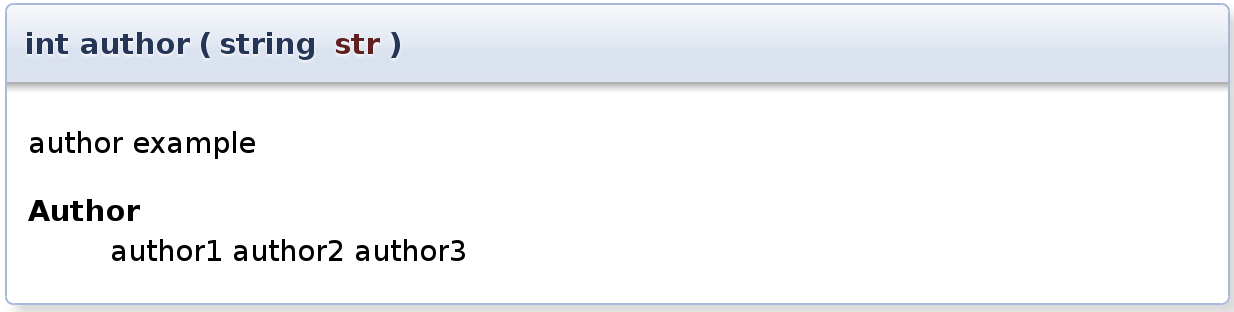
\includegraphics[width=0.8\textwidth]{image/write/document-the-code/developer-info/author-multi}
	\caption[فهرست نویسندگان]{
		فهرست نویسندگان.
	}
	\label{write/document-the-code/developer-info/author-multi}
\end{figure}


همانگونه که در نمونه بالا قابل مشاهده است، می‌توان فهرست تمام نویسندگان را با
استفاده از یک برچسب بیان کرد.
روش مناسب‌تر استفاده از این برچسب برای هر نویسنده است به این ترتیب نام
نویستنده‌گان هرکدام به صورت مستقل در یک خط نوشته می‌شود.
از این رو می‌توان نمونه بالا را به صورت زیر اصلاح کرد:
\begin{C++}
/**
 * \brief author example
 *
 * \author author1
 * \author author2
 * \author author3
 */
int author1(string str);
\end{C++}
مستند تولید شده برای این مستند در شکل \ref{write/document-the-code/developer-info/author-multi1}
نمایش داده شده است.
\begin{figure}
	\centering
	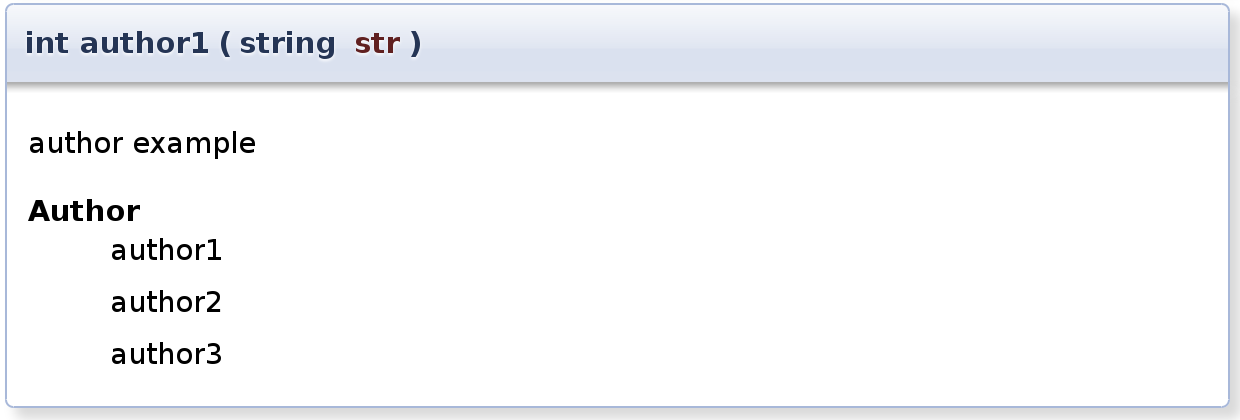
\includegraphics[width=0.8\textwidth]{image/write/document-the-code/developer-info/author-multi1}
	\caption[فهرست نویسندگان]{
		فهرست نویسندگان با به کاربردن چندین برچسب متوالی.
	}
	\label{write/document-the-code/developer-info/author-multi1}
\end{figure}

یک روش دیگر استفاده از برچسب \lr{authors} است.
تنها تفاوت میان این دو برچسب، عنوانی است که در خروجی تولید می‌شود.
با استفاده از برچسب \lr{authors} عنوان تولید شده در خروجی نیز به صورت جمع خواهد
بود در حالی که برچسب \lr{author} به صورت مفرد است.
به عنوان نمونه اصلاح نمونه بالا به صورت زیر مستند شکل
\ref{write/document-the-code/developer-info/author-multi2} را ایجاد می‌کند که
تنها در عنوان با یکدیگر متفاوت هستند.
\begin{C++}
/**
 * \brief author example
 *
 * \authors author1
 * \authors author2
 * \authors author3
 */
int authors(string str);
\end{C++}
\begin{figure}
	\centering
	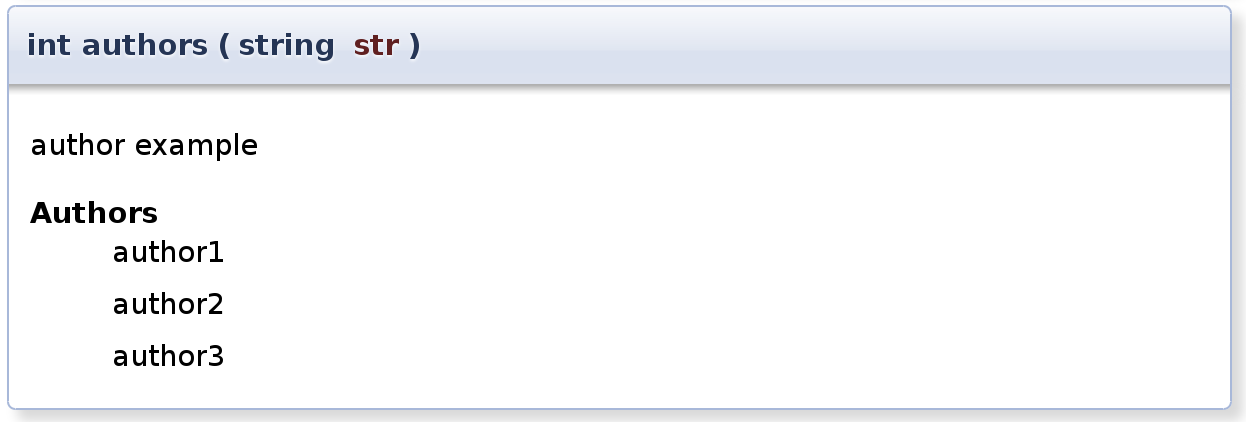
\includegraphics[width=0.8\textwidth]{image/write/document-the-code/developer-info/author-multi2}
	\caption[فهرست نویسندگان]{
		فهرست نویسندگان با استفاده از برچسب \lr{authors}.
	}
	\label{write/document-the-code/developer-info/author-multi2}
\end{figure}


\subsection{نسخه شروع}
% since
% \since { text }

در فرآیند توسعه سیستم‌ها، موجودیت‌های و امکانات متفاوت در برهه‌های زمانی و یا
نسخه‌های متفاوتی از سیستم ایجاد می‌شوند.
با استفاده از برچسب \lr{since} زمان اضافه شدن یک موجودیت به بسته اضافه تعیین می‌شود.
ساختار کلی این برچسب به صورت زیر است:
\begin{C++}
/**
 * \since { text }
 */
\end{C++}

در متن ورودی این برچسب، که در حالت کلی یک پاراگراف است، از ساختار خاصی استفاده نمی‌شود
و می‌توان تمام برچسب‌های زیباسازی متن را در آن به کار برد.
متن ورودی این برچسب با رسیدن به یک سطر خالی و یا برچسب‌های دیگر خاتمه می‌یابد.
برای نمونه فرض کنید که یک فراخوانی از نسخه ۲ یک بسته معرفی شده است، مستند مورد نیاز برای 
این فراخوانی، در ساده‌ترین حالت، به صورت زیر است:
\begin{C++}
/**
 * \brief since example
 *
 * \since 2.0.0 last update
 */
int since(string str);
\end{C++}

مستند ایجاد شده برای این نمونه در شکل \ref{write/document-the-code/developer-info/since} نمایش 
داده شده است.
\begin{figure}
	\centering
	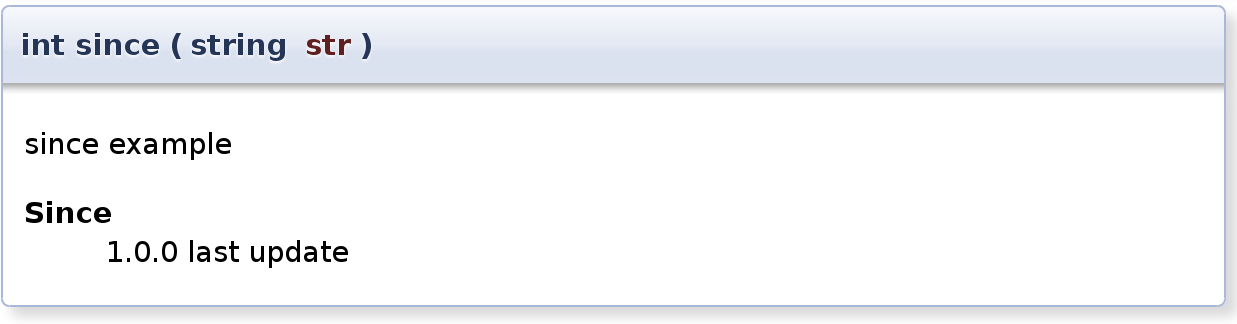
\includegraphics[width=0.8\textwidth]{write/document-the-code/developer-info/since}
	\caption[فهرست نویسندگان]{
		تعیین رویداد و یا نسخه‌ای اضافه شدن یک سیستم.
	}
	\label{write/document-the-code/developer-info/since}
\end{figure}

\begin{warning}
امکان استفاده از این برچسب بیش از یک بار برای هر موجودیت وجود دارد با این وجود این کار
از نظر مستند سازی کاملا اشتباه است.
ظهور یک امکان جدید تنها در یک زمان ممکن است و بعد از آن ممکن است دستخوش تغییراتی شده
و به روز شود.
برای نمایش تغییرات و به روز رسانی‌های از برچسب‌های دیگری مانند \lr{date}
\end{warning}

\subsection{کنارگذاشتن}
% deprecated
% \deprecated { description }

کنار گذاشتن و یا حذف یک امکان از سیستم در طول حیات آن بسیار معمول است.
در بسیاری از موارد امکانات ایجاد شده کارایی خود را از دست داده و یا با امکانات
جدید اضافه شده در تضاد هستند.
از این رو باید به ناچار آنها را کنار گذاشت و این موضوع را به نوعی به کاربران آن
سیستم انتقال داد.
اما سیستم‌ها باید به گونه‌ای توسعه یابند که با سازکارهای قدیم خود سازگار بوده و
سیستم‌های وابسته به خود را حمایت کنند.
نمی‌توان اینگونه تصور کرد که به محض کنار گذاشتن یک امکان از طراحی، در پیاده سازی
نیز باید آن را حذف کرد.

یک روش مناسب برای کنار گذاشتن یک امکان از سیستم، اعلام این کار در نسخه جاری و
اجرای آن در نسخه‌های آینده است.
در این روش امکان مورد نظر به صورت یک امکان کنار گذاشته معرفی می‌شود و در مستند
فنی به کاربران سیستم اعلام می‌شود.
در نهایت بعد از چند نسخه، بنا بر سیاست‌های توسعه، امکان مورد نظر به صورت کامل
حذف می‌شود.
در مستند سازی فنی از برچسب \lr{depricated} برای تعیین امکاناتی استفاده می‌شود که
در حال حاضر کنار گذاشته شده و در آینده نیز به صورت کامل از سیستم حذف می‌شود.
ساختار کلی این برچسب به صورت زیر است:
\begin{C++}
/**
 * \deprecated {description }
 */
\end{C++} 

از این برچسب برای تشریح ورش‌های جایگزین، زمان انقضا و حذف کامل و یا هر مستند
مورد نیاز برای موجودیت و یا امکان کنارگذاشته شده، استفاده می‌شود.
برای نمونه فرض کنید که یک فراخوانی در سیستم در نظر گرفته شده بوده است و در
طراحی به این نتیجه رسیده‌ایم که این فراخوانی باید حذف شود.
حداقل مستند مورد نیاز برای این فراخوانی به صورت زیر است:
\begin{C++}
/**
 * \brief deprecated example
 *
 * \deprecated This method will be removed in V2.0.1 completely, please use
 * deprecated2(string) instead.
 */
int deprecated(string str);
\end{C++}

در شکل \ref{write/document-the-code/developer-info/deprecated} خروجی تولید شده
برای این مستند نمایش داده شده است.
در فرآیند تولید مستند فنی، تمام موجودیت‌هایی که به عنوان یک موجودیت کنارگذاشته
شده تعیین می‌شوند در یک فهرست جمع آورده شده و به مستند اضافه می‌شود.
به این ترتیب با ارائه شدن یک نسخه جدید از سیستم و مستند فنی آن، کاربران
می‌توانند به سادگی فهرست تمام امکانات کنارگذاشته شده را مشاهده و تغییرهای مورد
نیاز را در سیستم‌های خود ایجاد کنند.
در شکل \ref{write/document-the-code/developer-info/deprecated-list} یک نمونه از
فهرست موجودیت‌های کنارگذاشده شده آورده شده است.
\begin{figure}
	\centering
	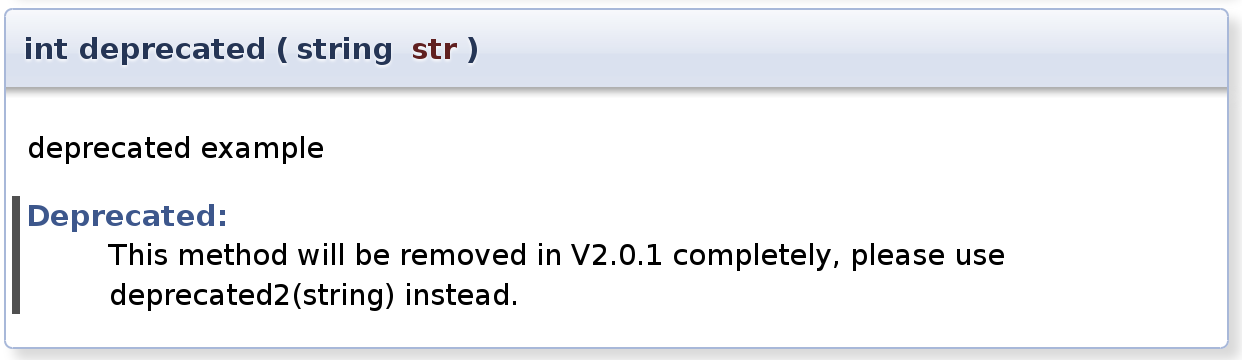
\includegraphics[width=0.8\textwidth]{image/write/document-the-code/developer-info/deprecated}
	\caption[موجودیت کنار گذاشته شده]{
		مستند یک موجودیت کنار گذاشته شده. در این مستند نه تنها روش جایگزین بلکه زمان
		حذف کامل این موجودیت نیز بیان شده است.
	}
	\label{write/document-the-code/developer-info/deprecated}
\end{figure}
\begin{figure}
	\centering
	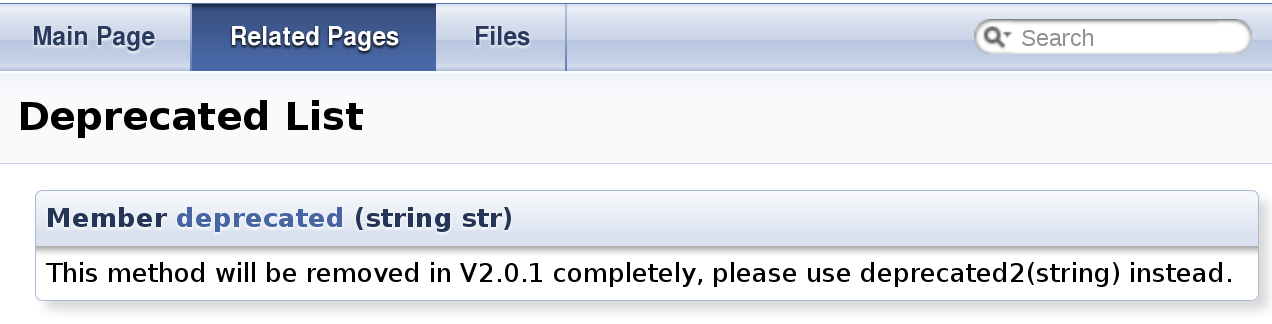
\includegraphics[width=0.8\textwidth]{write/document-the-code/developer-info/deprecated-list}
	\caption[فهرست موجودیت‌های کنار گذاشته شده]{
		فهرست تمام موجودیت‌های حذف شده. این فهرست کاربران را در توسعه و تغییر سیستم‌های خود
		یاری می‌کند.
	}
	\label{write/document-the-code/developer-info/deprecated-list}
\end{figure}


% \subsection{بخش}
% remarker
% \remark { remark text }
% 
% Starts a paragraph where one or more remarks may be entered. The paragraph will
% be indented. The text of the paragraph has no special internal structure. All
% visual enhancement commands may be used inside the paragraph. Multiple adjacent
% \remark commands will be joined into a single paragraph. Each remark will start
% on a new line. Alternatively, one \remark command may mention several remarks.
% The \remark command ends when a blank line or some other sectioning command is
% encountered.

